%%%%%%%%%%%%%%%%%%%%%%%%%%%%%%%%%%%%%%%%%%%%%%%%%%%%%%%%%%%%%%%%%%%%%%%%%%%%%%
%%
%% Dokumentacia k projektu 'Interpret pre jazyk IFJ 2013'
%%
%%
%%%%%%%%%%%%%%%%%%%%%%%%%%%%%%%%%%%%%%%%%%%%%%%%%%%%%%%%%%%%%%%%%%%%%%%%%%%%%%
\documentclass[12pt,a4paper,titlepage,final]{article}

% jazyk
\usepackage[slovak]{babel}
\usepackage[utf8]{inputenc}
% balicky prr odkazy
\usepackage[bookmarksopen,colorlinks,plainpages=false,urlcolor=blue,unicode]{hyperref}
\usepackage{url}
% obrazky
\usepackage[dvipdf]{graphicx}
% velikost stranky
\usepackage[top=3.5cm, left=2.5cm, text={17cm, 24cm}, ignorefoot]{geometry}

\setcounter{secnumdepth}{4}
\usepackage{pdflscape}
\usepackage{afterpage}
\usepackage{capt-of}% or use the larger `caption` package
\usepackage{amsmath}
\usepackage{rotating}
\newcommand{\BigO}[1]{\ensuremath{O\bigl(#1\bigr)}}
\newcommand{\ttlcb}{\texttt{\char 123}}
\newcommand{\ttrcb}{\texttt{\char 125}}
\newcommand{\ttsc}{\texttt{\char 59}}

\begin{document}

%%%%%%%%%%%%%%%%%%%%%%%%%%%%%%%%%%%%%%%%%%%%%%%%%%%%%%%%%%%%%%%%%%%%%%%%%%%%%%
% titulní strana

\def\projname{Okruh 4. Výrobný podnik}


\begin{titlepage}

% \vspace*{1cm}
\begin{figure}[!h]
  \centering
  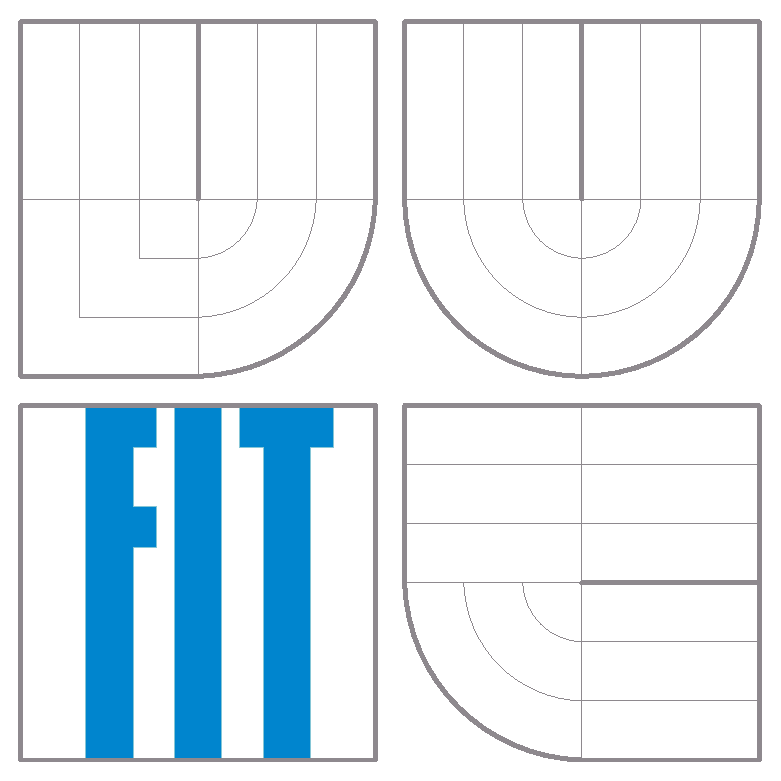
\includegraphics[height=5cm]{logo.eps}
\end{figure}
\center Fakulta Informačních Technologií \\
\center Vysoké Učení Technické v Brně \\

\vfill

\begin{center}
\bigskip
\begin{Huge}
\projname\\
\end{Huge}
\begin{large}
Modelovanie a simulácie\\
\end{large}
\end{center}

\vfill

\begin{center}
\begin{Large}
\today
\end{Large}
\end{center}

\vfill

\begin{flushleft}
\begin{large}
Marek Milkovič (xmilko01)\\
Lukáš Vrabec (xvrabe07) \\
\end{large}
\end{flushleft}
\end{titlepage}

%%%%%%%%%%%%%%%%%%%%%%%%%%%%%%%%%%%%%%%%%%%%%%%%%%%%%%%%%%%%%%%%%%%%%%%%%%%%%%
% obsah
\pagestyle{plain}
\pagenumbering{gobble}
\tableofcontents

%%%%%%%%%%%%%%%%%%%%%%%%%%%%%%%%%%%%%%%%%%%%%%%%%%%%%%%%%%%%%%%%%%%%%%%%%%%%%%
% textova zprava
\newpage
\pagestyle{plain}
\pagenumbering{arabic}
\setcounter{page}{1}

% sekcia 1
%%%%%%%%%%%%%%%%%%%%%%%%%%%%%%%%%%%%%%%%%%%%%%%%%%%%%%%%%%%%%%%%%%%%%%%%%%%%%%
\section{Úvod}
V tejto práci je riešená implementácia modelu hypotetického výrobného podniku
na produkciu základných dosiek, ktorá bude použitá pre vytvorenie simulačného
modelu systému.

Na základe modelu a simulačných experimentov bude ukázané chovanie systému
výrobného podniku v podmienkach rôzneho vyťaženia, pridávania jednotlivých
obslužních liniek.
TODO: scim experimentujeme. 

Cieľom experimentov je demonštrovanie možných optimalizácií na zadanom modely. Konkrétne
nájdenie optimálnejšej konfigurácie vzhľadom na počet vyrobených kusov základných 
dosiek ročne pri čo najmenšej veľkosti a cene výslednej výrobnej linky.

Pre spracovanie modelu je nutné naštudovať a pochopiť samotný proces výroby
základnej dosky(ďalej len výroby). Vyhľadať a spracovať informácie týkajúce sa 
technologií ktoré sú použité pri výrobe. Získať technické špecifikácie zariadení,
ktoré sa podieľajú na výrobe. Prispôsobenie modelovaného systému tak,
aby čo najviac odpovedal reálnemu systému výroby. Následne spracovať tieto údaje,
navrhnúť experimenty pré vytvorenie optimálnejších riešení výroby. 

%%%%%%%%%%%%%%%%%%%%%%%%%%%%%%%%%%%%%%%%%%%%%%%%%%%%%%%%%%%%%%%%%%%%%%%%%%%%%%
\subsection{Autori a zdroje faktov}
Na projekte sa podieľali študenti VUT FIT Marek Milkovič a Lukáš Vrabec. Informácie
a odborné fakty boli čerpané z internetu, odborných článkov a výročných
správ spoločností GIGA-BYTE Technology Co. Ltd. a ASUSTeK Computer Inc.
Všetky zdroje sú uverejnené na konci tohto dokumentu.

\subsection{Overenie validity modelu}
Validita modelu bola overovaná porovnávaním dát z dostupných zdrojov s výstupmi
simulácie. Pri vytváraní modelu boli čiastočne použité dôverihodné informácie,
pre nedôverihodné alebo nedostupné informácie boli zvolené hypotetické hodnoty,
ktoré približne odpovedajú reálnemu systému. 

% sekcia 2
%%%%%%%%%%%%%%%%%%%%%%%%%%%%%%%%%%%%%%%%%%%%%%%%%%%%%%%%%%%%%%%%%%%%%%%%%%%%%%
\section{Rozbor témy a použitých metód}
%%%%%%%%%%%%%%%%%%%%%%%%%%%%%%%%%%%%%%%%%%%%%%%%%%%%%%%%%%%%%%%%%%%%%%%%%%%%%%
Výrobný podnik spracováva požiadavky na výrobu základných dosiek, ktorý pracuje
v nepretržitej prevádzke. Prvým krokom v procese výroby je vstup dosiek plošných
spojov (\textit{angl.} printable circuit board, ďalej len PCB) do SMT
(\textit{angl. surface mount-technology}) liniek, kde dochádza k osadeniu jednotlivých
SMD (\textit{angl. surface-mount device}) komponent (rezistory, chipset atď.).
SMT linky sa skladajú zo zariadenia pre sieťotlač spájkovacej 
hmoty (\textit{angl. solder paste screen printer}) kde dochádza k nanášaniu spájkovacej
hmoty na PCB. Tento proces je vykonávaný 2 až 150 mm/sec [link]. Ďalej pokračuje
do P\&P (\textit{angl. Pick-and-Place}) prístroja ktorý na PCB umiestni 
SMD komponenty. Rýchlosť umiestnia SMD komponent na PCB je 0.25 až 0.5 sekundy
na čip [link]. Osadené komponenty je nutné upevniť. K tomuto účelu sa použije
pec ktorá pri vysokých teplotách upevní komponenty (spájkovanie pretavením), 
trvanie približne 5 minút v závisloti na použitom materiále. 

Proces pokračuje kontrolou nanometrových chýb spojov na PCB. Tento proces je 
nazývaný AOI (\textit{angl. automated optical insepction}). V prípade výskytu
chýb je PCB nutné manuálne opraviť. Po oprave je nutné AOI zopakovať. Tento
úkon nieje časovo náročny [link].

Následne je PCB umiestnená na DIP (\textit{angl. Dual in-line package})
linku ktorú predstavuje posuvný pás na ktorom sú manuálne umiesňované 
DIP konektory (DIMM,PCI-Express atď.). DIP konetkory sú upevnené v špeciálnej
peci (spájkovanie vlnou).

Proces výroby základnej dosky je hotový. Vykoná sa viacero manuálnych aj automatizovaných
testov. V prípade chýb je základná doska manuálne opravovaná a sú na nej opakovane vykonané
testy.

Posledným krokom je zabalenie základnej dosky, ktorá je pripravená na distribúciu.

Výrobný podnik môže obsahovať niekoľko SMT, DIP, testovích a baliacích liniek.

\subsection{Popis použitých postupov}
Simulačný model je konzolová aplikácia, naprogramovaná v programovacom jazyku
C++, podľa požiadaviek zadania. Simulačná knižnica SIMLIB/C++ bola použitá pretože
umožnuje objektovo zapísať model, čím je implementácia jednoduchšia a efektívnejšia.
Z tejto knižnice boli použité aj simulačné nástroje na zber štatistík. Na tvorbu
tabuliek a grafov bol použitý tabuľkový procesor Microsoft Excel.

\subsection{Popis pôvodu použitých metód}
Bola použitá knižnica SIMLIB/C++, v ktorej sme rozšírili model zariádení a 
skladov o identifikáciu v ktorej výrobnej linke sa nachádza.

% sekcia 3
%%%%%%%%%%%%%%%%%%%%%%%%%%%%%%%%%%%%%%%%%%%%%%%%%%%%%%%%%%%%%%%%%%%%%%%%%%%%%%
\section{Koncepcia modelu}
%%%%%%%%%%%%%%%%%%%%%%%%%%%%%%%%%%%%%%%%%%%%%%%%%%%%%%%%%%%%%%%%%%%%%%%%%%%%%%

% sekcia 4
%%%%%%%%%%%%%%%%%%%%%%%%%%%%%%%%%%%%%%%%%%%%%%%%%%%%%%%%%%%%%%%%%%%%%%%%%%%%%%
\section{Architektúra simulačného modelu}
%%%%%%%%%%%%%%%%%%%%%%%%%%%%%%%%%%%%%%%%%%%%%%%%%%%%%%%%%%%%%%%%%%%%%%%%%%%%%%

% sekcia 5
%%%%%%%%%%%%%%%%%%%%%%%%%%%%%%%%%%%%%%%%%%%%%%%%%%%%%%%%%%%%%%%%%%%%%%%%%%%%%%
\section{Simulačné experimenty a ich priebeh}
%%%%%%%%%%%%%%%%%%%%%%%%%%%%%%%%%%%%%%%%%%%%%%%%%%%%%%%%%%%%%%%%%%%%%%%%%%%%%%

% sekcia 6
%%%%%%%%%%%%%%%%%%%%%%%%%%%%%%%%%%%%%%%%%%%%%%%%%%%%%%%%%%%%%%%%%%%%%%%%%%%%%%
\section{Zhrnutie simulačných experimentov a záver}
%%%%%%%%%%%%%%%%%%%%%%%%%%%%%%%%%%%%%%%%%%%%%%%%%%%%%%%%%%%%%%%%%%%%%%%%%%%%%%


\end{document}
